% Grégoire
% Intro

%%%%
% 1 - Notre équipe a travaillé sur le projet 4 consistant
% en l'élaboration d'un bureau partagé. Cette courte
% présentation a pour objectif de vous expliquer les 
% problèmes que nous avons rencontrés et les résultats
% que nous avons obtenu. 
% 2 - Nous allons donc parler de phase de spécifications
% et de conception, des choix technologiques que nous avons 
% fait et des améliorations possibles pour le projet. Vous
% aurez ensuite droit à une démonstration.
% 3 - Pour introduire le sujet, permettez-moi de revenir sur
% la notion de bureau partagé. On parle souvent de VNC. Un VNC,
% c'est un système de controle de l'environnement de bureau
% d'un autre ordinateur. Je vous ai mis ici un exemple sous KDE.
% Nous avons choisi de le comprendre autrement.
% Pour nous, un bureau partagé, c'est un environnement de
% bureau collaboratif, à partager avec des copains.
% Elisoa va vous expliquer tout ça plus en détails en vous
% présentant les spécifications.


\begin{frame}
	\frametitle{Un bureau partagé ? }
	\begin{figure}
		\centering
		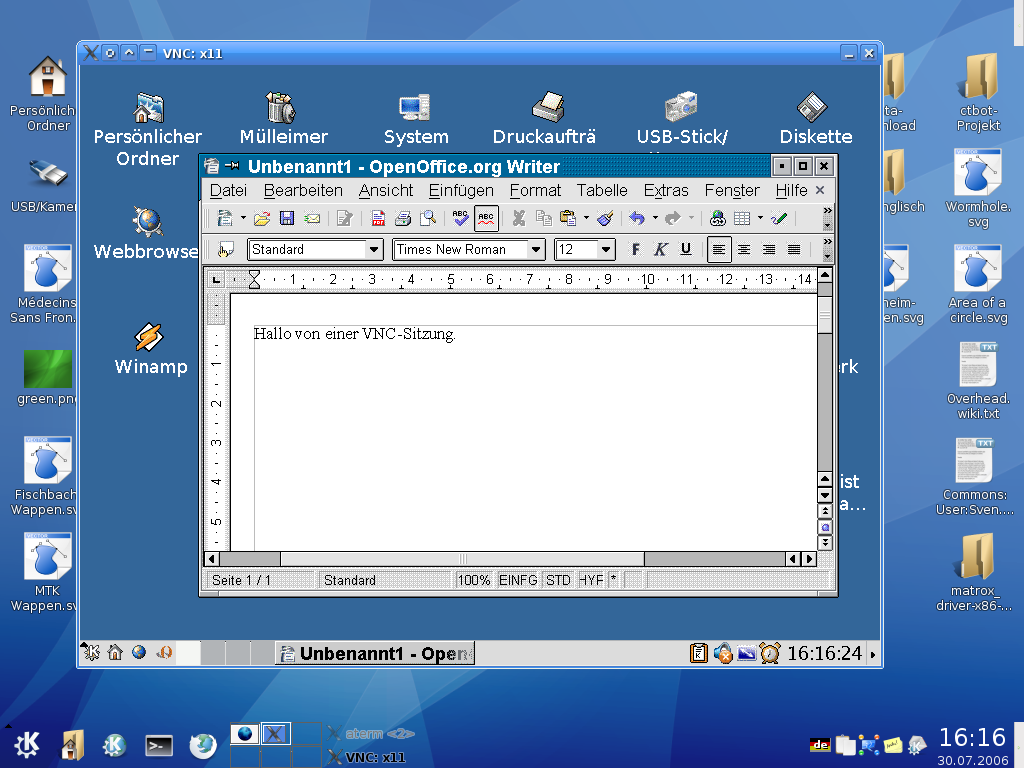
\includegraphics[scale=0.22]{resources/VNC.png}
		\caption{Un exemple de bureau partagé dans KDE 3}
	\end{figure}
\end{frame}